\section{Introduction}
Let $M$ be a stable matching. For any man $m$ let $s_M(m)$ denote the first woman $w$ on $m$ 's list such that $w$ strictly prefers $m$ to $p_M(w)$ (her partner in $M$ ). Let next $_M(m)$ denote the partner in $M$ of woman $s_M(m)$. Note that since $M$ is stable, $m$ prefers $p_M(m)$ to $s_M(m)$. Note also that $s_M(m)$ might not exist. For example, if $M$ is the woman optimal matching, then $s_M(m)$ does not exist for any man.

\begin{exmp}\label{exmp_3_1}
Consider the stable matching $M_1$ from Figure \ref{FIG_2_2}. 

\begin{center}
    $\begin{array}{lll}1: & 3 & 2 \\ 2: & 8 & 1 \\ 3: & 1 & 6 \\ 4: & 8 & 1 \\ 5: & 2 & 7 \\ 6: & 5 & 3 \\ 7: & 5 & 3 \\ 8: & 2 & 7\end{array}$

    \begin{figure}[ht]
  \centering
  \caption{Woman $s_{M_1}(m)$ and man $\operatorname{next}_{M_1}(m)$ for each man $m$}
  \label{FIG_3_1}
\end{figure}
\end{center}
\end{exmp}

There is another way to think about $s_M(m)$ and $\operatorname{next}_M(m)$ that is motivated by the extended version of the Gale-Shapley algorithm discussed earlier. Suppose for each woman $w$ we delete all pairs $\left(m^{\prime}, w\right)$ such that $w$ prefers $p_M(w)$ to $m^{\prime}$. It is easy to see that in the resulting lists, which we call reduced lists, $p_M(w)$ is the last entry in $w$'s list, and $s_M(m)$ is the entry just following $p_M(m)$ in $m$ 's list. It is also true that $p_M(m)$ is the first entry in $m$'s list (hence $s_M(m)$ is the second entry), for if any woman $w^{\prime}$ remains above $p_M(m)$ after the deletions, then $w^{\prime}$ prefers $m$ to her partner in $M$, and $\left(m, w^{\prime}\right)$ would block $M$. So, after the deletions, $p_M(m)$, $s_M(m)$, and $p_M(w)$ are easy to identify, and $\operatorname{next}_M(m)$ is also easy to find, since it is the last entry on $p_M(m)$ 's new list; equivalently, $\operatorname{next}_M(m)$ is the man $m^{\prime}$ such that $p_M(m)$ is the first entry on the reduced list of $m^{\prime}$.

Note that when $M=M_0$, the reduced lists are the MGS-lists defined and discussed in the previous chapter. The use of reduced lists will streamline the presentation of certain algorithms to be discussed later.

\begin{center}
    $\begin{array}{llllll}
    1: & 8 & 3 & & & \\ 2: & 3 & 6 & & & \\ 3: & 5 & 1 & 6 & 2 & \\ 4: & 6 & 8 & 5 & & \\ 5: & 7 & 2 & 1 & 3 & 6 \\ 6: & 1 & 5 & 2 & 3 &  \\ 7: & 2 & 5 & 7 & 8 & 1 \\ 8: & 4 & 2 & 6 & &\end{array}$
    \begin{figure}[ht]
  \centering
  \caption{The reduced lists of the men for stable matching $M_1$}
  \label{FIG_3_2}
\end{figure}
\end{center}

 As an example, Figure \ref{FIG_3_2} shows the reduced lists of the men when $M$ is the stable matching $M_1$ of Figure \ref{FIG_2_2}.

Let $\rho=\left(m_0, w_0\right),\left(m_1, w_1\right), \ldots,\left(m_{r-1}, w_{r-1}\right)$ be an ordered list of pairs in a stable matching $M$ such that for each $i(0 \leq i \leq r-1), m_{i+1}$ is $\operatorname{next}_M\left(m_i\right)$, where $i+1$ is taken modulo $r$. Then $\rho$ is called a rotation (exposed) in $M$, and we say that $m$ (or $w$ ) is in rotation $\rho$ if there is a pair $(m, w)$ in the ordered list defining $\rho$. From this point on, it will be assumed that whenever we refer to an element $m_i$ or $w_i$ in a rotation $\left(m_0, w_0\right),\left(m_1, w_1\right), \ldots,\left(m_{r-1}, w_{r-1}\right)$, the value of the subscript $i$ is taken modulo $r$.

\begin{exmp}\label{exmp_3_2}
    It is easy to see from Figure \ref{FIG_3_2} that the ordered list of pairs $(1,8),(2,3),(4,6)$ is an exposed rotation in matching $M_1$, as is the ordered list $(3,5)$, $(6,1)$. There are no other rotations exposed in $M_1$.
\end{exmp}

Note that a rotation may be exposed in more than one matching, and hence the definition does not associate a rotation with a unique matching. However, no ordered set of pairs is a rotation unless it satisfies the above definition for at least one stable matching of $\mathcal{M}$. As a first indication of the utility of rotations, and their connection to minimal differences, we prove the following.

\begin{lemma}\label{lem_3_1}
If $\rho=\left(m_0, w_0\right),\left(m_1, w_1\right), \ldots,\left(m_{r-1}, w_{r-1}\right)$ is a rotation, and for some $i \quad(0 \leq i \leq$ $r-1), w$ is any woman strictly between $w_i$ and $w_{i+1}$ in man $m_i$ 's list, then $\left(m_i, w\right)$ is not a stable pair, i.e., it is never a pair in any stable matching of $\mathcal{M}$.
\end{lemma}


\begin{proof}
Let $M$ be any stable matching in which $\rho$ is exposed. Then in $m_i$ 's list, $w$ is strictly between $w_i$ (which is $p_M\left(m_i\right)$ ) and $w_{i+1}$ (which is $s_M\left(m_i\right)$ ), and by the definition of $s_M\left(m_i\right), w$ prefers her partner in $M$ to $m_i$. Now suppose $\left(m_i, w\right)$ is a pair in stable matching $M^{\prime}$. Then both $m_i$ and $w$ prefer their partners in $M$ to their partners in $M^{\prime}$, violating Theorem earlier proven.
\end{proof}

\begin{exmp}\label{exmp_3_3}
    In rotation $(1,8),(2,3),(4,6)$, which is exposed in matching $M_1$ of Figure \ref{FIG_2_2},$m_0$ is man 1 , and woman 4 is between woman $w_0(8)$, and woman $w_1(3)$. So, the pair $(1,4)$ cannot be in any stable matching for the preferences of Figure \ref{FIG_2_1}.
\end{exmp}

If $M$ is a stable matching, and $\rho=\left(m_0, w_0\right),\left(m_1, w_1\right), \ldots,\left(m_{r-1}, w_{r-1}\right)$ is a rotation exposed in $M$, then $M / \rho$ is defined to be the matching in which each man not in $\rho$ stays married to his partner in $M$, and each man $m_i$ in $\rho$ marries $w_{i+1}=s_M\left(m_i\right)$. The matching $M / \rho$ essentially differs from $M$ by a one place cyclic shift of each man in $\rho$ to the $M$-partner of the next man in $\rho$; hence it is easy to verify that it is a matching, i.e., it is one-one. The transformation of $M$ to $M / \rho$ is called the elimination of $\rho$ from $M$.

\begin{exmp}\label{exmp_3_4}
    The elimination of rotation $(1,8),(2,3),(4,6)$ from $M_1$ yields the matching $M_2$ of Figure \ref{FIG_2_2} , and the elimination of $(3,5),(6,1)$ from $M_1$ yields $M_3$.
\end{exmp}

The following two central lemmas further demonstrate the utility of rotations; for example, they immediately imply that $M_0$ can be transformed to $M_z$ through a sequence of stable matchings, by successively finding and eliminating any exposed rotation in each successive matching.

\begin{lemma}\label{lem_3_2}
    If $\rho$ is any rotation exposed in a stable matching $M$, then $M / \rho$ is a stable matching dominated by $M$.
\end{lemma}

\begin{proof}
    Suppose $(m, w)$ blocks $M / \rho$. All the women either have the same or better partners in $M / \rho$ than in $M$, and $w$ prefers $m$ to her partner in $M / \rho$, so she also prefers $m$ to her partner in $M$. But then $m$ must be in $\rho$ or else $(m, w)$ would block $M$. So $w$ is strictly above $s_M(m)$ in $m$ 's list and she prefers $m$ to $p_M(w)$, contradicting the definition of $s_M(m)$ as the first woman in $m$ 's list who prefers $m$ to her partner in $M$.
\end{proof}


\begin{lemma}\label{lem_3_3}
    If $M$ is any stable matching other than the woman optimal matching $M_z$, then there is at least one rotation exposed in $M$.
\end{lemma}


\begin{proof}
    Let $m$ be any man who has different partners in $M$ and $M_z$, and let $w$ be $m$ 's partner in $M_z$. Since $M_z$ is woman-optimal and man-pessimal, $m$ strictly prefers his partner in $M$ to $w$, and $w$ strictly prefers $m$ to her partner in $M$. Hence $s_M(m)$ exists. Also, if $s_M(m)$ exists and $m^{\prime}=\operatorname{ext}_M(m)$ (the partner in $M$ of woman $s_M(m)$ ), then $s_M\left(m^{\prime}\right)$ exists also. Otherwise, $m^{\prime}$ and $s_M(m)$ would be partners in $M_z$, so $m$ would prefer $s_M(m)$ to his partner in $M_z$, and $s_M(m)$ would prefer $m$ to her partner in $M_z$, contradicting the stability of $M_z$.

    Now let $H(M)$ be a directed graph with a node for each man $m$ who has different partners in $M$ and $M_z$. Direct an edge from the node for $m$ to the node for $\operatorname{ext}_M(m)$, which, as shown above, must also be in $H(M)$. Then, every node in $H(M)$ has out-degree exactly one, and so there must be a simple cycle in $H(M)$. Any such simple cycle defines the men in a rotation exposed in $M$, in the order that they appear in the rotation; for any man $m$ in the cycle, $\left(m, p_M(m)\right)$ is a pair in the associated rotation.
\end{proof}

\begin{figure}[h]
  \centering
  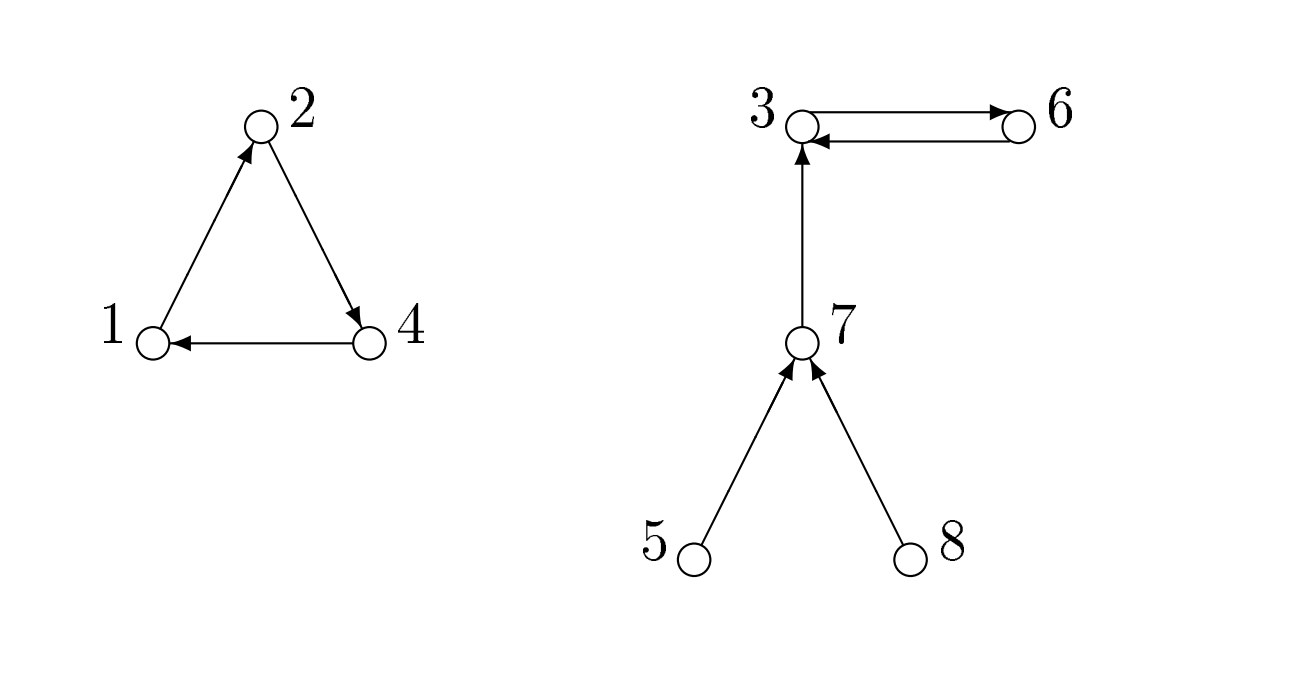
\includegraphics[width=0.65\textwidth]{IMAGES_FIGS/FIG_2_7.png}
  \caption{The graph $H(M)$}
  \label{FIG_3_3}
\end{figure}

The above proof gives a simple way to find a rotation exposed in $M$: starting from any man $m$, traverse the \textit{unique} path in $H(M)$ from $m$ until $m$ or some other node is visited twice. If $\rho$ is the rotation discovered by this traversal, we say that $m$ leads to rotation $\rho$; if $m$ leads to $\rho$ but is not in $\rho$, then the path in $H(M)$ from $m$ to the first man in $\rho$ is called a \textbf{tail} of $\rho$. Note that a rotation can have several tails. 

\begin{corollary}\label{cor_3_1}
If $m$ has different partners in $M$ and $M_z$, then $m$ leads to exactly one exposed rotation in $M$, so $m$ is either in exactly one rotation exposed in $M$ or is in exactly one tail.
\end{corollary}

The following lemma is an extension of Lemma \ref{lem_3_1} and is proved in essentially the same way.

\begin{lemma}\label{lem_3_4}
    If $\rho$ is exposed in $M$ and $m$ is a man on a tail of $\rho$ in $H(M)$, then $(m, w)$ cannot be a stable pair if $w$ is strictly between $p_M(m)$ and $s_M(m)$.
\end{lemma}

